\documentclass[journal,12pt,onecolumn]{IEEEtran}

% Import necessary packages
\usepackage{cite}
\usepackage{amsmath,amssymb,amsfonts,amsthm}
\usepackage{algorithmic}
\usepackage{graphicx}
\usepackage{textcomp}
\usepackage{xcolor}
\usepackage{txfonts}
\usepackage{listings}
\usepackage{enumitem}
\usepackage{mathtools}
\usepackage{gensymb}
\usepackage{comment}
\usepackage[breaklinks=true]{hyperref}
\usepackage{tkz-euclide} 
\usepackage{listings}
\usepackage{gvv}                                        
\usepackage[latin1]{inputenc}                                
\usepackage{color}                                            
\usepackage{array}                                            
\usepackage{longtable}                                       
\usepackage{calc}                                             
\usepackage{multirow}                                         
\usepackage{hhline}                                           
\usepackage{ifthen}                                           
\usepackage{lscape}
\usepackage{tabularx}
\usepackage{array}
\usepackage{float}
\usepackage{multicol} % Add the multicol package
\usepackage{circuitikz}
\usepackage{textcomp}
% New theorem declarations
\newtheorem{theorem}{Theorem}[section]
\newtheorem{problem}{Problem}
\newtheorem{proposition}{Proposition}[section]
\newtheorem{lemma}{Lemma}[section]
\newtheorem{corollary}[theorem]{Corollary}
\newtheorem{example}{Example}[section]
\newtheorem{definition}[problem]{Definition}

% Custom command definitions
\newcommand{\BEQA}{\begin{eqnarray}}
\newcommand{\EEQA}{\end{eqnarray}}
\newcommand{\define}{\stackrel{\triangle}{=}}

\theoremstyle{remark}
\newtheorem{rem}{Remark}

% Document begins here
\begin{document}
\bibliographystyle{IEEEtran}
\vspace{3cm}

% Title of the document
\title{ASSIGNMENT 5}
\author{EE24BTECH11011 - PRANAY}
\maketitle

\bigskip

% Custom figure and table numbering
\renewcommand{\thefigure}{\theenumi}
\renewcommand{\thetable}{\theenumi}
   \begin{enumerate}\setcounter{enumi}{13}
   \item A function $y\brak{t}$ , such that $y\brak{0}=1$ and $y\brak{1} = 3e^{-1}$, is a solution of the differential equation $\frac{d^2 y}{dx^2} + 2\frac{dy}{dx}+y =0$. Then $y\brak{2}$ is
   \begin{multicols}{4}
       \begin{enumerate}
           \item $5e^{-1}$
           \item $5e^{-2}$
           \item $7e^{-1}$
           \item $7e^{-2}$
       \end{enumerate}
   \end{multicols}
   \item The value of the integral
   \begin{align}
       \oint_c \frac{2z+c}{\brak{z - \frac{1}{z}}+\brak{z^2 - 4z + 5}} dz
   \end{align}
   over the contour $\abs{z} = 1$, taken in anticlockwise direction,would be
   \begin{multicols}{4}
       \begin{enumerate}
           \item $\frac{24 \pi i}{13}$
           \item $\frac{48 \pi i}{13}$
           \item $\frac{24 }{13}$
           \item $\frac{12}{13}$
       \end{enumerate}
   \end{multicols}
   \item The transfer function of a system is $\frac{Y\brak{s}}{R\brak{s}} = \frac{s}{s+2}$. Then the steady state output $y\brak{t}$ is $A\cos{\brak{2t + \varphi}}$ for the input $\cos{\brak{2t}}$.Then the values of $A$ and $\varphi$ ,respectively are
   \begin{multicols}{4}
       \begin{enumerate}
           \item $\frac{1}{\sqrt{2}},-45\degree$
           \item $\frac{1}{\sqrt{2}},+45\degree$
           \item ${\sqrt{2}},+45\degree$
           \item ${\sqrt{2}},-45\degree$
       \end{enumerate}
   \end{multicols}
   \item The phase cross-over frequency of the transfer function $G\brak{s} = \frac{100}{\brak{s+1}^3}$ in rad/s is
   \begin{multicols}{4}
       \begin{enumerate}
           \item $\sqrt{3}$
           \item $\frac{1}{\sqrt{3}}$
           \item $3$
           \item $3\sqrt{3}$
       \end{enumerate}
   \end{multicols}
   \item Consider a continous-time system with input $x\brak{t}$ and output $y\brak{t}$ given by 
   \begin{align}
       y\brak{t} = x\brak{t}\cos{t}
   \end{align}
   This system is
   \begin{enumerate}
       \item linear and time-invariant
       \item non-linear and time-invariant
       \item linear and time-varying
       \item non-linear and time-varying\\
   \end{enumerate}
   \item The value of $\int_{-\infty}^{+\infty} e^{-t} \delta\brak{2t-2}dt$, where $\delta \brak{t}$ is the Dirac delta function,is
   \begin{multicols}{4}
       \begin{enumerate}
           \item $\frac{1}{2e}$
           \item $\frac{2}{e}$
           \item $\frac{1}{e^2}$
           \item $\frac{1}{2e^2}$
       \end{enumerate}
   \end{multicols}
   \item A temperature in the range of $-40\degree\text{C}$ to $55\degree\text{C}$ is to
   be measured with a resistance of $0.1\degree\text{C}$.The minimum number of ADC bits required to get a matching dynamic range of the temperature sensor is
   \begin{multicols}{4}
       \begin{enumerate}
           \item $8$
           \item $10$
           \item $12$
           \item $14$
       \end{enumerate}
   \end{multicols}
   \item Consider the following unit which uses $2-\text{to}-1$ multiplier as shown in the figure.The boolean expression for output $F$ in terms of $A$ and $B$ is
 \begin{center}

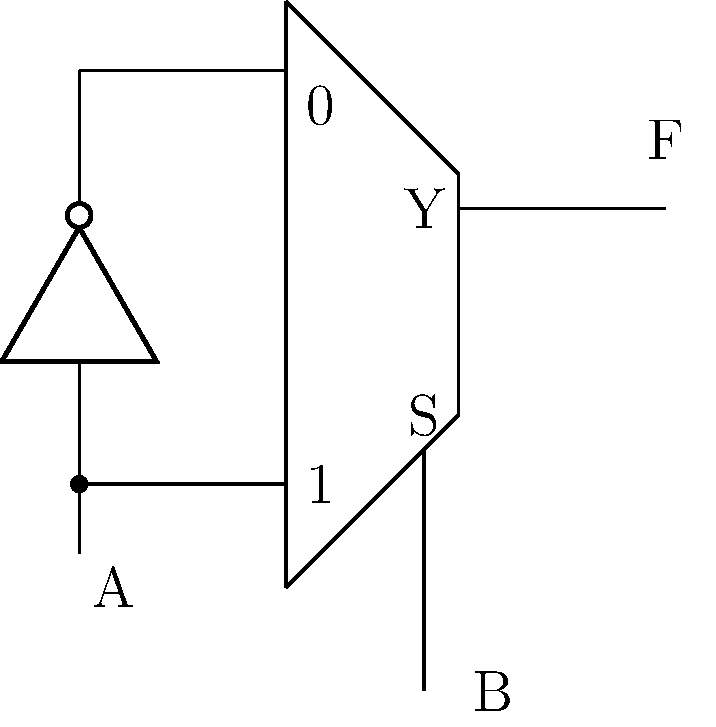
\includegraphics[width=0.2\textwidth]{figs/fig1/main} 
\end{center}
 
	   
   \begin{multicols}{4}
       \begin{enumerate}
           \item $A \oplus B$ \item $\overline{A+B}$ \item $A+B$ \item $\overline{A \oplus B}$
       \end{enumerate}
   \end{multicols}
   \item A transistor circuit is given below. The Zener diode breakdown volatge is $5.3$ V as shown. Take base to emitter volatge drop to be $0.6$V. The value of the current gain $\beta$ is \rule{3cm}{0.15mm}
 \begin{center}

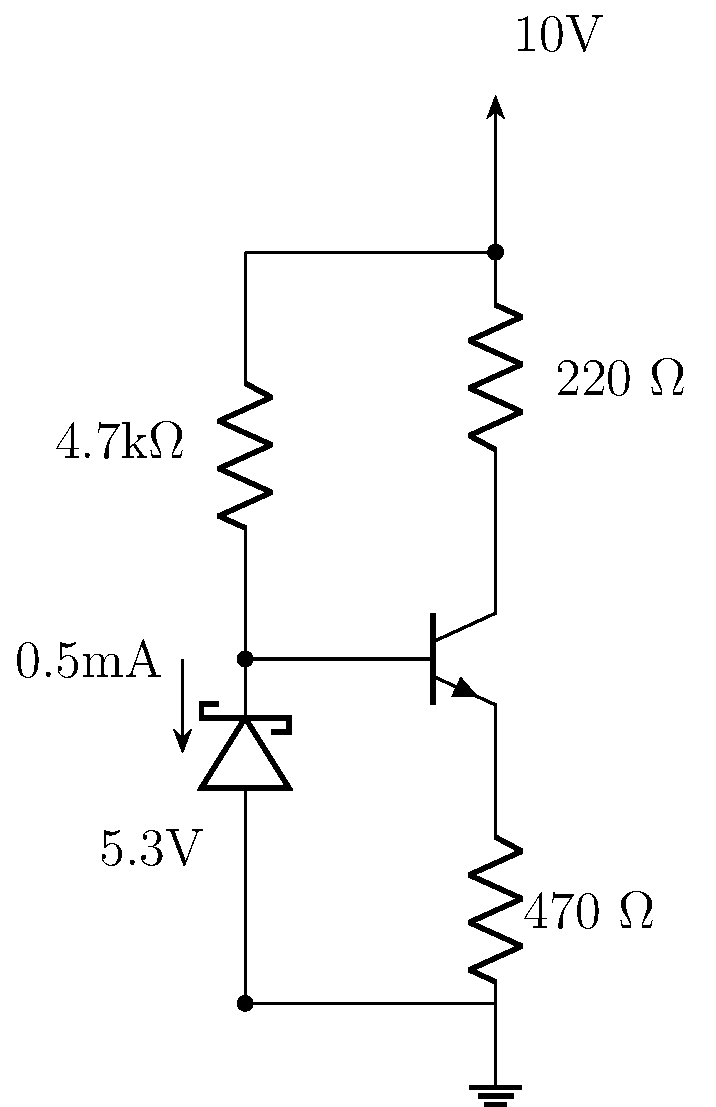
\includegraphics[width=0.25\textwidth]{figs/fig2/main} 
\end{center}
	   
   \item In cylindrical coordinate system , the potential produced by a uniform ring charge is given by $\varphi = f\brak{r,z}$ where $f$ is a continous fraction of $r$ and $z$. Let $\vec{E}$ be the resulting electric field. Then the magnitude of $\nabla \times \vec{E}$
   \begin{enumerate}
       \item increases with $r$
       \item is $0$
       \item is $3$
       \item decreases with $z$
   \end{enumerate}
   \item A soft-iron toroid is concentric with a long straight conductor carrying a direct current $I$. If the relative permeability $\mu_r$ of soft-iron is $100$, the ratio of the magnetic flux densities at two adjacent points located just inside and just outside the toroid, is \rule{3cm}{0.15mm}\\
   \item $R_A$ and $R_B$ are the input resistances of circuits as shown below.The circuits extend infinitely in the direction shown. Which one of the following statements is TRUE?
 \begin{center}

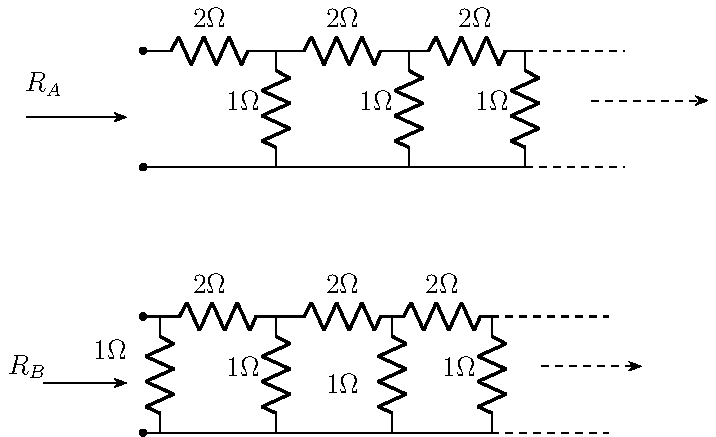
\includegraphics[width=0.6\textwidth]{figs/fig3/main} 
\end{center}
	   
   \begin{multicols}{4}
       \begin{enumerate}
           \item $R_A = R_B$
           \item $R_A = R_B = 0$
           \item $R_A < R_B$
           \item $R_B = \frac{R_A}{1+R_A}$
       \end{enumerate}
       \end{multicols}
       \item In a constant $\frac{V}{f}$ induction motor drive , the slip at maximum torque
       \begin{enumerate}
           \item is directly proportional to the synchronous speed
           \item remains constant with respect to the synchronous speed
\item  has an inverse relation with the synchronous speed
\item has no relation with the synchronous speed
       \end{enumerate}

       \end{enumerate}
       \end{document}
